%! TEX root = 'main.tex'

\section{Design}
\label{sec:design}

In this section, we present the design of our project. It has two major parts, the main module setups SMAP environment, monitors kernel to user space accesses, intercepts and handles related page faults and makes the page attributes transitioning. The other part is the hypervisor. As briefly mentioned in the introduction, the hypervisor in charges of isolating the SMAP feature to certain processes.

\subsection{Monitoring Kernel to User Space Accesses}

This is the major issue we faced when addressing kernel TOCTOU vulnerability. Reading and writing memory is the most common operation that a computer system does. So even with virtualization technology, there is no trap event on accessing memory. However, what makes the kernel TOCTOU vulnerability special is the fact that it's always the case that the kernel accesses user space. So we employ SMAP to monitor such behavior. 

Because there is no reasons for the user parameters to change during the ongoing syscall, we should make them unchangeable. For now, due to the practical reason that SMAP works on page granularity, we protect all the pages that contain the user parameters from being tampered with. Conflicts caused by this will be solved later in this section.

As mentioned earlier, once SMAP enabled, kernel accessing user space triggers page fault exceptions, so we intercepts OS's page fault handler. But the handler needs to handle all the exceptions in the system, it's a efficiency critical component. So the first thing we need to do is to distinguish the ones that caused by SMAP or by our subsequent protection. Notice that SMAP is a very strict rule. For example, in Linux system, the two user-data-access functions copy\_to\_user() and copy\_from\_user() temporarily disable SMAP right before accessing user space and re-enable it right after. That means the system should not seen any SMAP caused exception. Once there is one, the Linux kernel will take it as a serious error, then panic. The same with Windows, it didn't support SMAP yet, it also crashes when sees such exceptions.

Even though Intel provides two new instructions CLAC/STAC to temporarily disable/enable the feature, in page fault handler, it's already too late to cancel it.

Now we have a efficient hardware mechanism that can inform us whenever there is a kernel-to-user access. The rest is to protect the pages and to let the system continue. We choose to put the faulting page into the kernel space by setting the attributes in theirs page table entries(PTE). By doing so, the page fault exception is handled because it's no longer kernel accessing a user page, also the faulting page is protected from other user threads. 

\subsection{Page Attribute Transition} % transition or conversion? Or something else?


The memory management unit(MMU) in x86 architecture use page tables to map between virtual and physical pages~\cite{intelpaging}. Every page in the virtual memory has corresponding page table entries. As shown in~\autoref{fig:pte}, it contains bits that describes the page. For example, whether a page belongs to kernel or user depends on the 'User/Supervisor' bit. If the bit is set, then this page is a user page; if not, it's a kernel page. Obviously, user pages can be accessed by both user code and kernel code, but kernel pages can only be accessed by kernel code. 

\begin{figure}[th]
  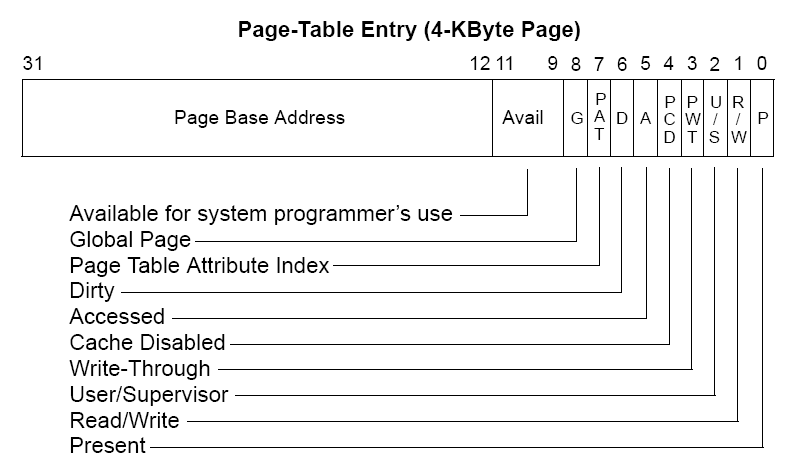
\includegraphics[width=0.47\textwidth]{figures/pte}
  \centering
  \caption{U/S, the 'User/Supervisor' bit, controls access to the page based on privilege level. If the bit is set, then this page is considered in user mode space and be accessed by all code; if the bit is not set, then it's considered in kernel mode space and can be accessed only by kernel mode code. }
  \label{fig:pte}
\end{figure}


When handling a page fault exception, the faulting virtual address is always stored in the CR2 register and the root of the current process's page tables is stored in CR3 register. First we need to walk through the page table to locate the corresponding page table entry of the faulting address. Then to put a user page into kernel space, simply changes the 'U/S' bit to 0. It becomes a kernel page even thought it's address doesn't look so, because normally on x86 Windows system, the kernel space is above address 0x80000000. We also can change it back by doing the opposite with the 'U/S' bit. We do so when the current syscall ends.

When the page is in kernel space, it's protected from user code accesses, as shown in~\autoref{fig:denyuserwrite}.

\begin{figure}[th]
  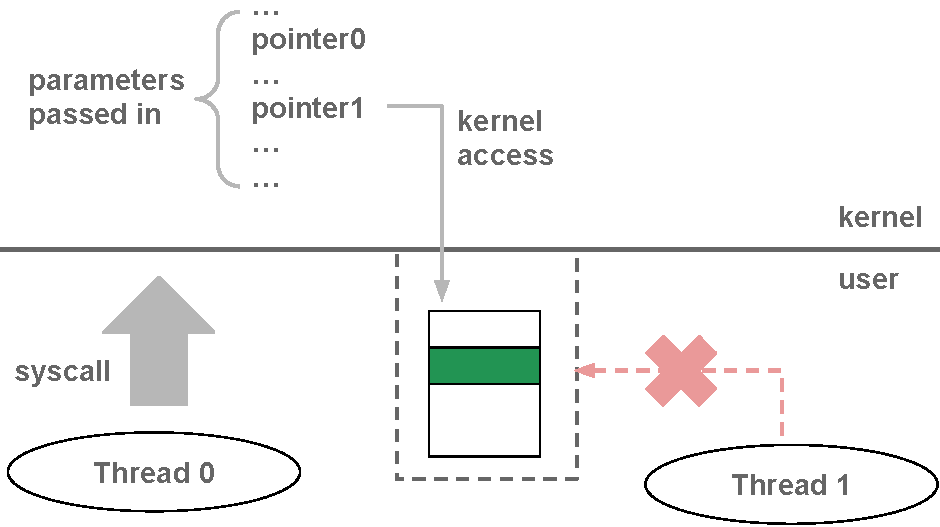
\includegraphics[width=0.47\textwidth]{figures/denyuserwrite}
  \centering
  \caption{}
  \label{fig:denyuserwrite}
\end{figure}


This is the base of our model. In reality, it's common that other user threads try to access data within the same page. For example, global variables or heap data when threads share the same heap pool. Even there are cases where read-only data is merged into one section with code by the compiler. We need to handle these situations as well.

To address this issue, user reading and user writing should be treated separately. Because reading doesn't change any data, it's safe to our mitigation. So when reading happens, we changes the page back to user space in order to fulfill the request. But we still want to remain its protection, because once we put it back, before another kernel access, this page is subject to any user access including writing. The solution is setting the page as read-only as well so subsequent writing triggers exception too. Certainly we record those information so when handling write violation we could behave accordingly and later restore the page attribute correctly. ~\autoref{fig:pagestate} shows the transitions due to different causes. 


\begin{figure}[th]
  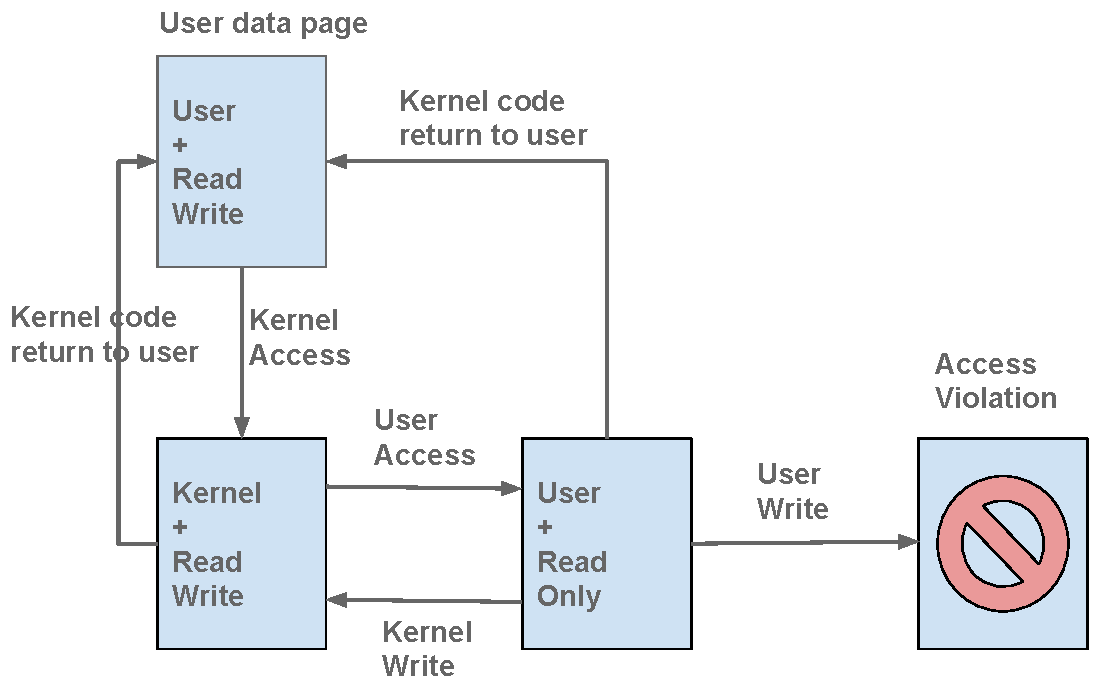
\includegraphics[width=0.45\textwidth]{figures/pagestate}
  \centering
  \caption{Page attributes transit between kernel mode and user mode. When kernel mode code ends, for example, system service returns to user mode, the page will be set back to the original permission}
  \label{fig:pagestate}
\end{figure}


Kernel reads/writes and user reads make the page transit from spaces and change attributes. The challenge remain is to handle user writes. 


\subsection{Handling Write Conflicts}
Subject to the x86 architecture, the hardware mechanism works only on page granularity, meaning one page can't be partially protected. So our approach is the following. Since pages only need to be protected during the ongoing syscall, when a thread tries to write data during the time, we make the thread wait until the ongoing syscall ends. More specifically, the thread waits inside the page fault handler, giving up it's CPU time slice. 

\begin{figure}[th]
  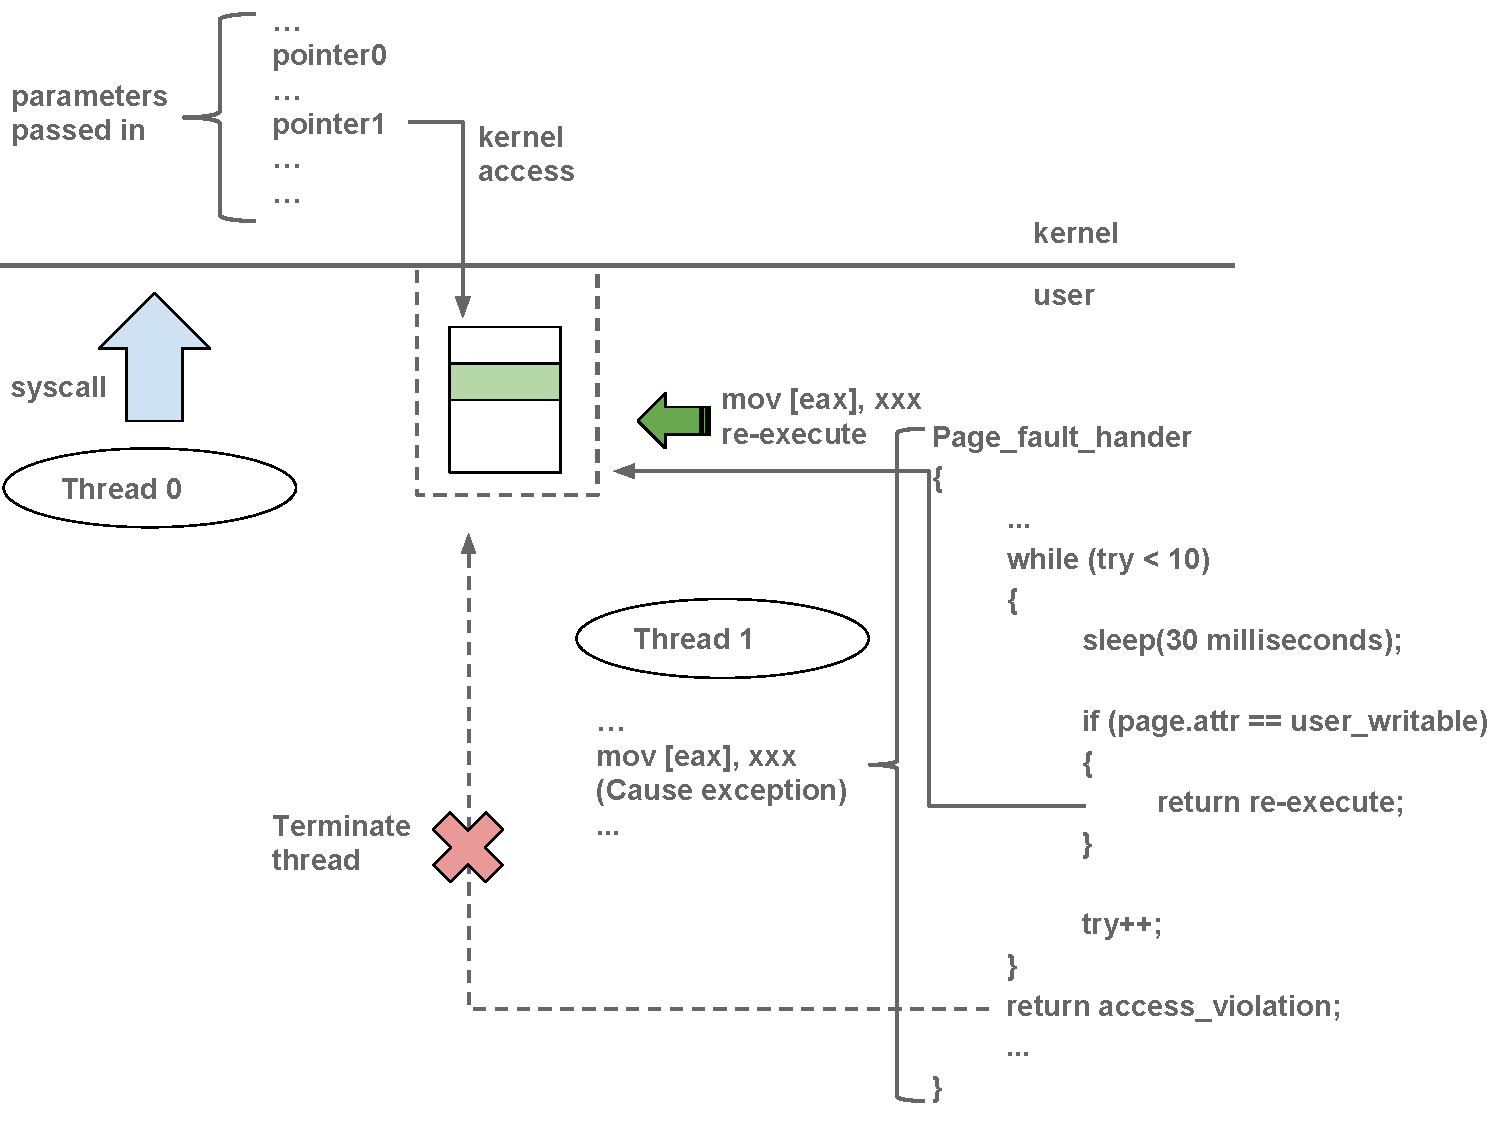
\includegraphics[width=0.47\textwidth]{figures/reexecute}
  \centering
  \caption{}
  \label{fig:reexecute}
\end{figure}


As shown in~\autoref{fig:reexecute}, thread 0 invoke a syscall. The kernel gets data from a user page, because of the mitigation, this page is protected. Then thread 1 tries to write it. It causes a page fault exception. From the error code our page fault handler is able to tell that this is a writing request, so it can't be granted. By calling a windows kernel function KeDelayExecutionTread(), the current thread gets into "sleep". After certain amount of time, it wakes up and checks if the page is released. If so, the page fault handler finish this exception and re-execute the faulting instruction. Otherwise, it sleeps again. A retry threshold is set in order to avoid deadlocks, for example, after ten tries, the thread will be terminated.  

\subsubsection{The Differences Between Interrupt and Exception}

Sleeping inside the page fault handler sounds strange. To explain it, I should briefly talk about what are exception and interruption and what's the difference.

Interrupt is a signal emitted by a peripheral hardware device such as network card, telling CPU that the device needs immediate attention. It's also called external interrupt or hardware interrupt(There is also software interrupt, but not discussed here). They have higher priority than the OS's scheduler and even higher than most of the kernel components. It's not suitable to put time consuming job in the interrupt handler. Any job that takes too long may even trigger the watchdog crash~\cite{msdnwatchdog}.   

On the other hand, exception is generated internally by the CPU, informing the OS to handle an event or an error, such as double fault, page fault, general protection fault and etc. In x86 architecture, external interrupts and exceptions are all handled through the Interrupt Descriptor Table(IDT), they all part of the kernel code. But unlike external interrupt, exception's priority is the same level with the OS scheduler. In Windows system's terminology, the Interrupt Request Level(IRQL) stays at PASSIVE\_LEVEL which also is the level where user program runs. So it's possible to safely call Windows kernel function KeDelayExecutionThread(), which has similar effect as a user program calls sleep(). 


\subsection{Releasing Protected Pages}

Whenever a syscall ends, all the protected page that related to it should be released. Their original attributes will be restored. The Thread Environment Block(TEB) is used to identify each thread within the current process. Each thread has its own TEB data and it's address is easy to locate by segment register FS. 

We hook a Windows internal function in order to know when it's the end of the syscall. 

\begin{comment}
\begin{figure}[th]
  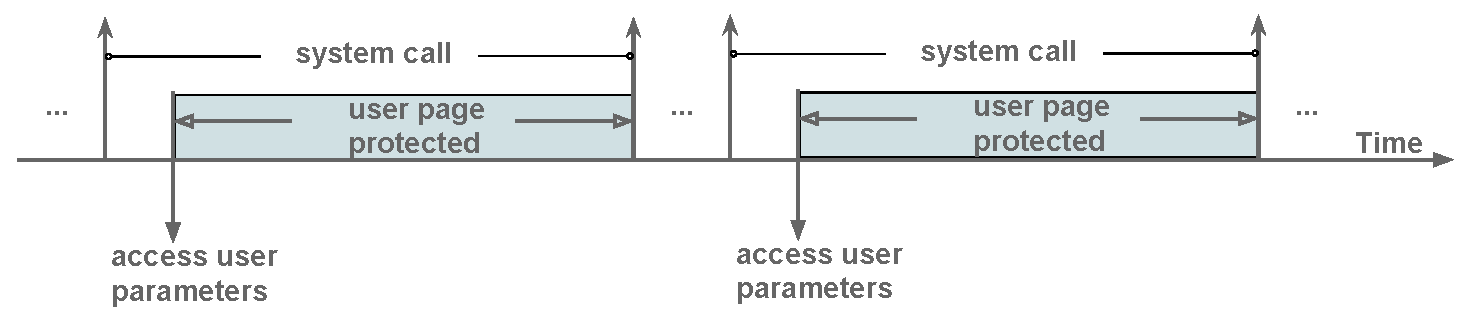
\includegraphics[width=0.47\textwidth]{figures/timeline}
  \centering
  \caption{The page protection period is within one system call cycle, this is based on the fact that kernel TOCTOU vulnerability does not happen across system calls.}
  \label{fig:timeline}
\end{figure}
\end{comment}



\subsection{TLB Caching}


\subsection{Hypervisor}

In the experiment, when we first enable SMAP in Windows system, exceptions flooded. Because Windows is not regulated itself as SMAP required, so every process, almost every syscall triggers SMAP page fault exception. And there is no easy way to simply discard them, even attached debugger is froze. To make it possible to just focus one case at a time, we figured a mechanism that can isolate SMAP inside a small range is necessary.

Eventually we chose to use virtualization technology, a hypervisor, to isolate a CPU feature such as SMAP into particular processes. Even though hypervisor costs performance overhead, but in cloud computing environment nowadays, hypervisor is already in the settings.

Hypervisor or virtual machine monitor(VMM) has several types. For example, native or bare-metal hypervisor, these hypervisors run directly on the host's hardware to control the hardware and to manage guest operating systems. Xen, Microsoft Hyper-V and VMware ESXi are this kind. Hosted hypervisor, these hypervisors run on a conventional operating system just as other programs do. VMware Workstation and QEMU are examples of this type.

But the one we use is none of these. It's a very simple runtime hypervisor. It doesn't emulate any hardware device but just monitors events of the system~\cite{howtohide}. Intel's virtualization technology makes it possible to transfer a running system from non-virtualization environment into the VMM guest mode. Our hypervisor is loaded as a Windows kernel driver at runtime. It sets up and enters virtualization, lifts the running OS into guest mode, and itself becomes the hypervisor.  

Also based on efficiency considerations, page fault handling is a highly optimized component. It's meaningful to reduce exceptions that being introduced by SMAP. As mentioned earlier, not all processes in the system need to be monitored. So the hypervisor framework is also one contribution of this paper. 

SMAP is enabled when the SMAP bit in the CR4 is set. So the idea is to set it during the particular process. In x86 architecture, VMM provides virtual memory space for every process and each process may have multiple threads that share the same virtual memory space. Each process has a set of page tables that maps virtual pages to physical pages. So the root of the page table is stored in CR3. Every time a process switches in or out, the CR3 will be set correspondingly.

Fortunately, Intel's virtualization technology allows us to capture that event. Operation on control registers cause the virtual machine (VM, the OS in guest mode in this case)to exit to the root mode(hypervisor). For example, "MOV CR3, EAX" is a typical instruction when setting the CR3, where EAX has the new page table root. Every time when the system does that, our hypervisor gets a chance to get involved.

\begin{figure}[th]
  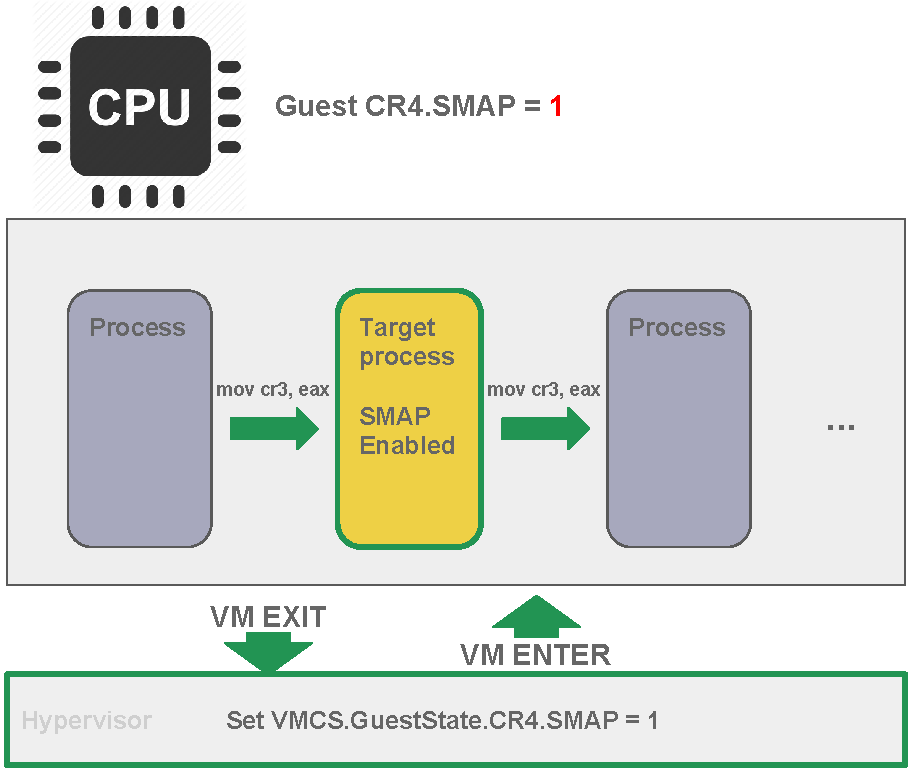
\includegraphics[width=0.47\textwidth]{figures/processmap}
  \centering
  \caption{SMAP is only enabled on the target process. In other words, only target process can trigger SMAP exceptions.}
  \label{fig:processmap}
\end{figure}

Suppose we focus on one particular process, as shown in~\autoref{fig:processmap}, when VM exits, compares the new CR3 with the our targeted one, if they match, we will set the SMAP bit in the CR4 field of the virtual machine control structure(VMCS) of the VM. This is the structure which is used to update the real hardware registers when re-entering the virtual machine. Therefore, when the VM resumes, the processor's CR4 will be updated. Because this is the current process that is running, it will feel that SMAP is enabled. When this process switches out, we clears SMAP bit. So SMAP will be disable for other processes.

